\documentclass[12pt,english,dvipsnames,aspectratio=169,handout]{beamer}\usepackage[]{graphicx}\usepackage[]{xcolor}
% maxwidth is the original width if it is less than linewidth
% otherwise use linewidth (to make sure the graphics do not exceed the margin)
\makeatletter
\def\maxwidth{ %
  \ifdim\Gin@nat@width>\linewidth
    \linewidth
  \else
    \Gin@nat@width
  \fi
}
\makeatother

\definecolor{fgcolor}{rgb}{0.345, 0.345, 0.345}
\newcommand{\hlnum}[1]{\textcolor[rgb]{0.686,0.059,0.569}{#1}}%
\newcommand{\hlstr}[1]{\textcolor[rgb]{0.192,0.494,0.8}{#1}}%
\newcommand{\hlcom}[1]{\textcolor[rgb]{0.678,0.584,0.686}{\textit{#1}}}%
\newcommand{\hlopt}[1]{\textcolor[rgb]{0,0,0}{#1}}%
\newcommand{\hlstd}[1]{\textcolor[rgb]{0.345,0.345,0.345}{#1}}%
\newcommand{\hlkwa}[1]{\textcolor[rgb]{0.161,0.373,0.58}{\textbf{#1}}}%
\newcommand{\hlkwb}[1]{\textcolor[rgb]{0.69,0.353,0.396}{#1}}%
\newcommand{\hlkwc}[1]{\textcolor[rgb]{0.333,0.667,0.333}{#1}}%
\newcommand{\hlkwd}[1]{\textcolor[rgb]{0.737,0.353,0.396}{\textbf{#1}}}%
\let\hlipl\hlkwb

\usepackage{framed}
\makeatletter
\newenvironment{kframe}{%
 \def\at@end@of@kframe{}%
 \ifinner\ifhmode%
  \def\at@end@of@kframe{\end{minipage}}%
  \begin{minipage}{\columnwidth}%
 \fi\fi%
 \def\FrameCommand##1{\hskip\@totalleftmargin \hskip-\fboxsep
 \colorbox{shadecolor}{##1}\hskip-\fboxsep
     % There is no \\@totalrightmargin, so:
     \hskip-\linewidth \hskip-\@totalleftmargin \hskip\columnwidth}%
 \MakeFramed {\advance\hsize-\width
   \@totalleftmargin\z@ \linewidth\hsize
   \@setminipage}}%
 {\par\unskip\endMakeFramed%
 \at@end@of@kframe}
\makeatother

\definecolor{shadecolor}{rgb}{.97, .97, .97}
\definecolor{messagecolor}{rgb}{0, 0, 0}
\definecolor{warningcolor}{rgb}{1, 0, 1}
\definecolor{errorcolor}{rgb}{1, 0, 0}
\newenvironment{knitrout}{}{} % an empty environment to be redefined in TeX

\usepackage{alltt}
\usepackage{fontspec}
\setsansfont[Mapping=tex-text]{Fira Sans}
\setcounter{secnumdepth}{4}
\setcounter{tocdepth}{4}
\usepackage[normalem]{ulem}
\usepackage[T1]{fontenc}
\usepackage{dcolumn}
\usepackage{booktabs}
\usepackage{bm}
\usepackage{setspace}
\makeatletter
\usetheme{metropolis}
\setbeamertemplate{frame footer}{Bosancianu | Schaub | Hertie School}
\setbeamerfont{page number in head/foot}{size=\tiny}
\setbeamercolor{footline}{fg=gray}
\usepackage{xcolor}
\setbeamercovered{dynamic}
\usepackage{tikz}
\usetikzlibrary{arrows, positioning, fit, shapes, shapes.misc}
\usepackage[labelformat=empty]{caption}
% For table captions in Beamer
\usepackage[sectionbib]{apacite}
\renewcommand{\bibliographytypesize}{\footnotesize}
\makeatletter
\let\st@rtbibsection\@bibnewpage
\let\st@rtbibchapter\@bibnewpage
\makeatother
\usepackage{amsmath, mathtools}
\usepackage{xunicode}
\usepackage{hyperref}
\graphicspath{{./figures/}} 
% Defines a checkmark
\def\checkmark{\tikz\fill[scale=0.4,color=orange](0,.35) -- (.25,0) -- (1,.7) -- (.25,.15) -- cycle;}
% Code for circles in Table cells
\newcounter{nodemarkers}
\newcommand\circletext[1]{%
    \tikz[overlay,remember picture] 
        \node (marker-\arabic{nodemarkers}-a) at (0,1.5ex) {};%
    #1%
    \tikz[overlay,remember picture]
        \node (marker-\arabic{nodemarkers}-b) at (0,0){};%
    \tikz[overlay,remember picture,inner sep=2pt]
        \node[draw,ellipse,fit=(marker-\arabic{nodemarkers}-a.center) (marker-\arabic{nodemarkers}-b.center)] {};%
    \stepcounter{nodemarkers}%
}
% wide itemize and enumerate
\newenvironment{wideitemize}{\itemize\addtolength{\itemsep}{.3em}}{\enditemize}
\newenvironment{wideenumerate}{\enumerate\addtolength{\itemsep}{.3em}}{\endenumerate}
% boxes
\def\boxitorange#1{%
  \smash{\color{orange}\fboxrule=1pt\relax\fboxsep=2pt\relax%
  \llap{\rlap{\fbox{\vphantom{0}\makebox[#1]{}}}~}}\ignorespaces
}
\def\boxitblue#1{%
  \smash{\color{blue}\fboxrule=1pt\relax\fboxsep=2pt\relax%
  \llap{\rlap{\fbox{\vphantom{0}\makebox[#1]{}}}~}}\ignorespaces
}
\newcommand{\indep}{\perp \!\!\!\! \perp}
\setbeamertemplate{itemize items}{\checkmark}
\usepackage{multirow}
\hypersetup{pdfauthor={Bosancianu and Schaub},
	pdftitle={Statistical Modeling and Causal Inference with R},
	pdfsubject={Week 6: Matching},
	pdfkeywords={Berlin, Hertie, 2020, week 5}}
\title{\textsc{Statistical Modeling and Causal Inference with R}}
\subtitle{Week 6: Matching}
\date{October 12, 2020}
\author{Manuel Bosancianu \hfill Max Schaub}
\institute{Hertie School of Governance}
\IfFileExists{upquote.sty}{\usepackage{upquote}}{}
\begin{document}
\maketitle


\begin{frame}
	\frametitle{Lecture Q\&A}
	\begin{itemize} \large
		\item Open Q\&A 
		\item Boyd, Epstein, Martin \citeyear{boyd_untangling_2010}
	\end{itemize}
\end{frame}


\begin{frame}
	\frametitle{Boyd, Epstein, Martin \citeyear{boyd_untangling_2010}}
	\footnotesize
	\begin{enumerate}
		\item What is the research question?
		\item Why does the effect of the having a female judge on a panel lend itself to causal analysis, but not the effect of the sex of the judge herself? (And should the second question hence not be studied?)
		\item What is the role of ideology in what the authors call a) individual effects, and b) panel effects? Draw DAG, and explain.
		\item Is there an issue with common support?
		\item Which covariates do the authors control for/match on, and why? Is their strategy appropriate? Given the argument, what effect would you expect matching to have? 
	\end{enumerate}
\end{frame}


\begin{frame}
	\frametitle{Boyd, Epstein, Martin \citeyear{boyd_untangling_2010}: Ideology and the DAG}
	\footnotesize
  	 \begin{figure} 
    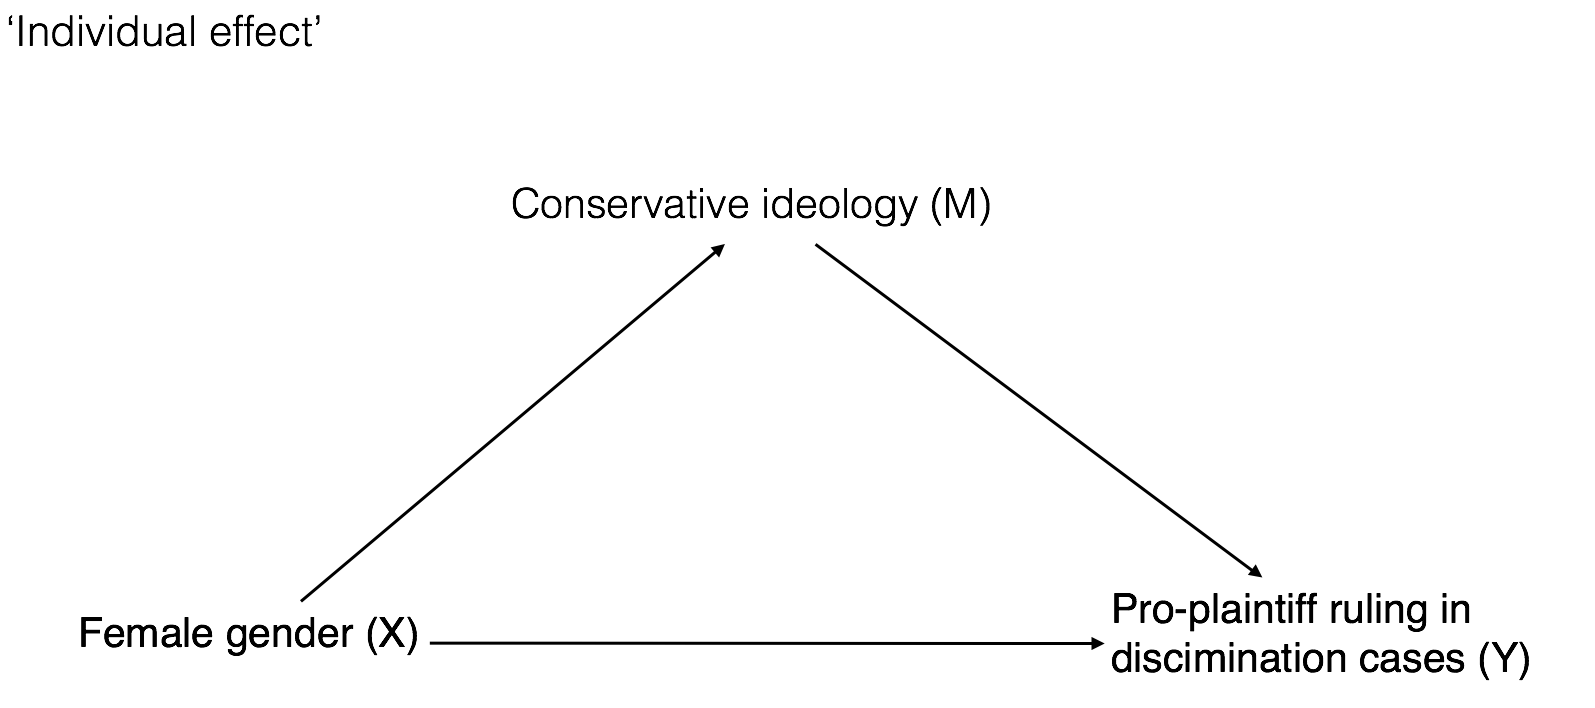
\includegraphics[height=.65\textheight,keepaspectratio=true]{../04-figures/06/03-w6_dag_ind}
    \end{figure}
    In `individual effect', ideology is mediator!
\end{frame}



\begin{frame}
	\frametitle{Boyd, Epstein, Martin \citeyear{boyd_untangling_2010}: Ideology and the DAG}
	\footnotesize
  	 \begin{figure} 
    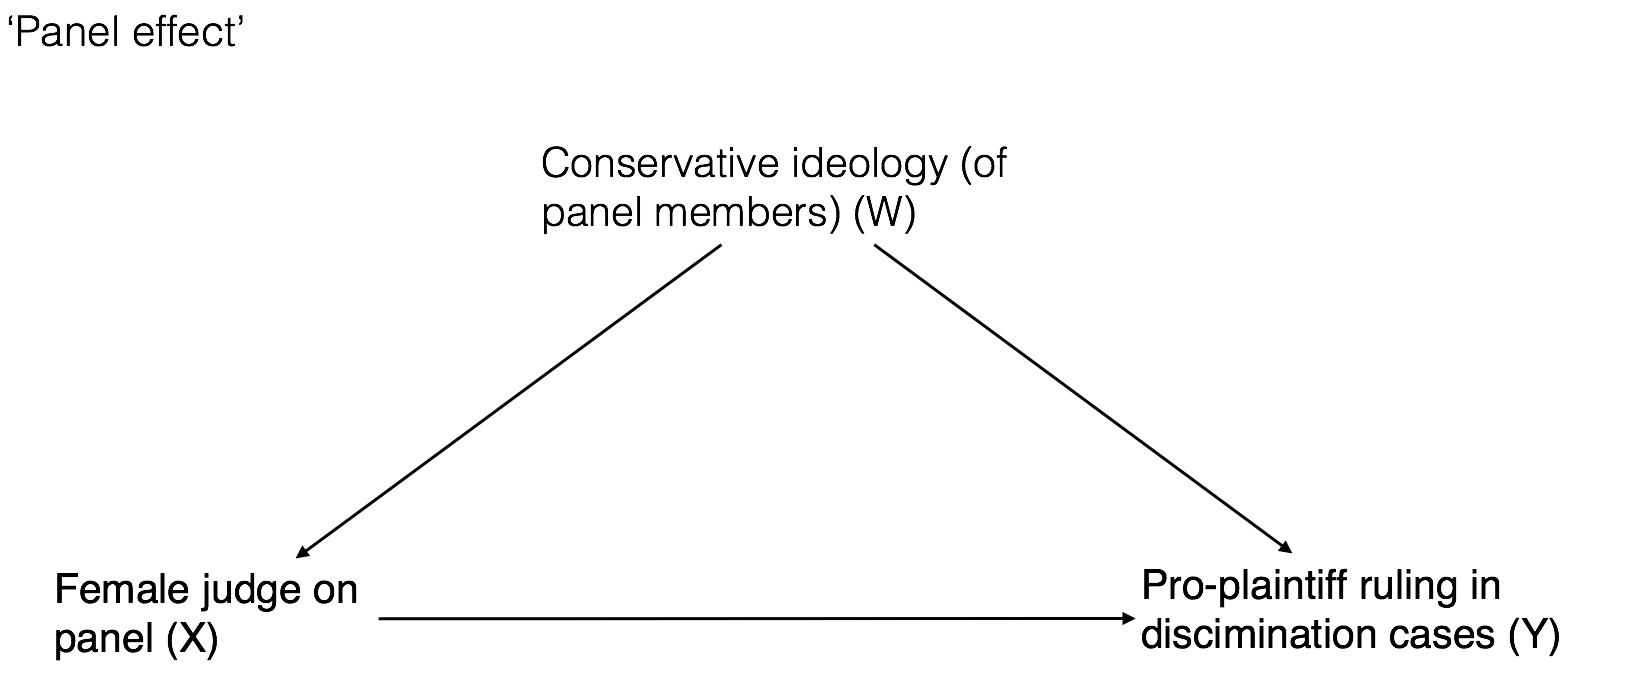
\includegraphics[height=.65\textheight,keepaspectratio=true]{../04-figures/06/04-w6_dag_panel}
    \end{figure}
    In `panel effect', ideology may be confounder
\end{frame}


\begin{frame}
	\frametitle{Boyd, Epstein, Martin \citeyear{boyd_untangling_2010}: Common support}
	\footnotesize
  Is there a lack of common support with regard to ideology?
  	 \begin{figure} 
    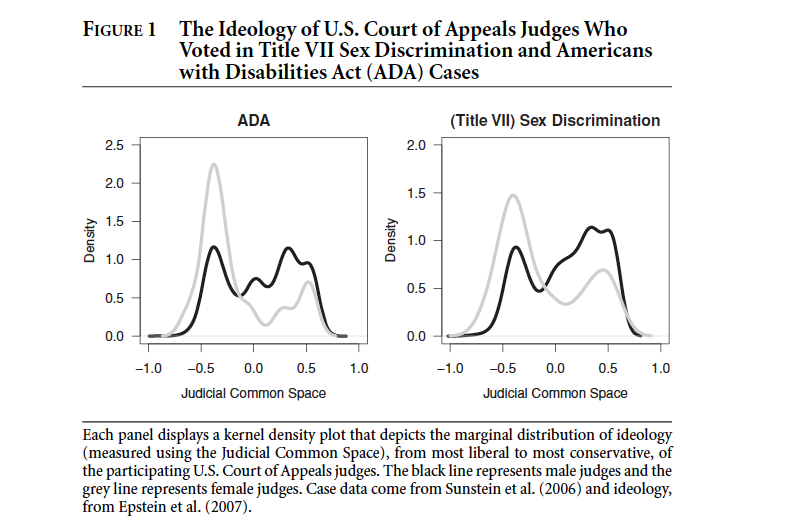
\includegraphics[height=.6\textheight,keepaspectratio=true]{../04-figures/06/05-w6_density}
    \end{figure}
\end{frame}


\begin{frame}
	\frametitle{Boyd, Epstein, Martin \citeyear{boyd_untangling_2010}: Common support}
	\footnotesize
  Figure demonstrating lack of common support
  	 \begin{figure} 
    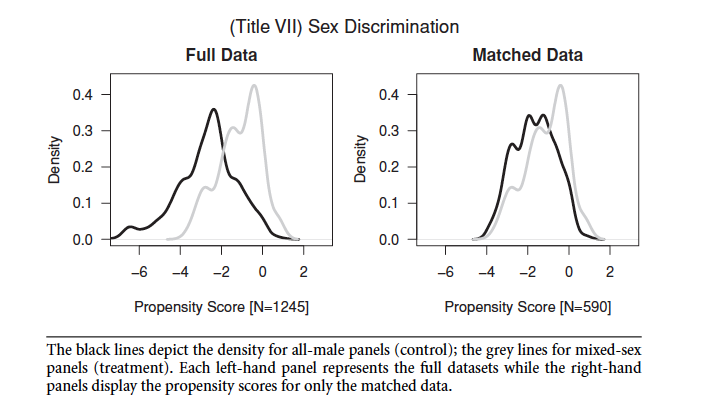
\includegraphics[height=.6\textheight,keepaspectratio=true]{../04-figures/06/06-w6_density2}
    \end{figure}
\end{frame}


\begin{frame}
	\frametitle{Boyd, Epstein, Martin \citeyear{boyd_untangling_2010}: Choosing controls}
	\footnotesize
	How should we determine which variables to control for? Is the the following selection warranted?
	\begin{itemize} \scriptsize
		\item ideology
		\item year of birth
		\item ideology
		\item minority judge
		\item judicial experience
		\item circuit dummies
	\end{itemize} \footnotesize
	Do these variables shut possible back doors? Do they reflect the assignment process? What variables would?
\end{frame}


\begin{frame}
	\frametitle{Boyd, Epstein, Martin \citeyear{boyd_untangling_2010}: Choosing controls}
	\footnotesize
  Panel assignment procedure for appellate courts
  	 \begin{figure} 
    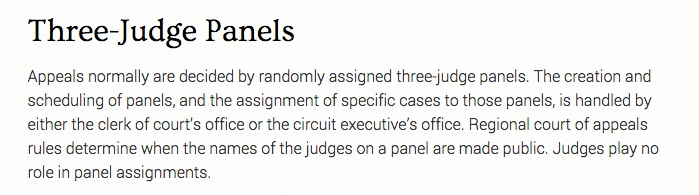
\includegraphics[height=.4\textheight,keepaspectratio=true]{../04-figures/06/07-w6_three_judge}
    \end{figure}
    \tiny
    \url{https://www.uscourts.gov/statistics-reports/appellate-courts-and-cases-journalists-guide\#panels}
    
    \footnotesize
    Given this assignment procedure, what would you control for/match on? And would you expect matching and multivariate regression estimates to differ? 
\end{frame}


\begin{frame}
	\frametitle{Boyd, Epstein, Martin \citeyear{boyd_untangling_2010}: Choosing controls}
	\footnotesize
  	 \begin{figure} 
    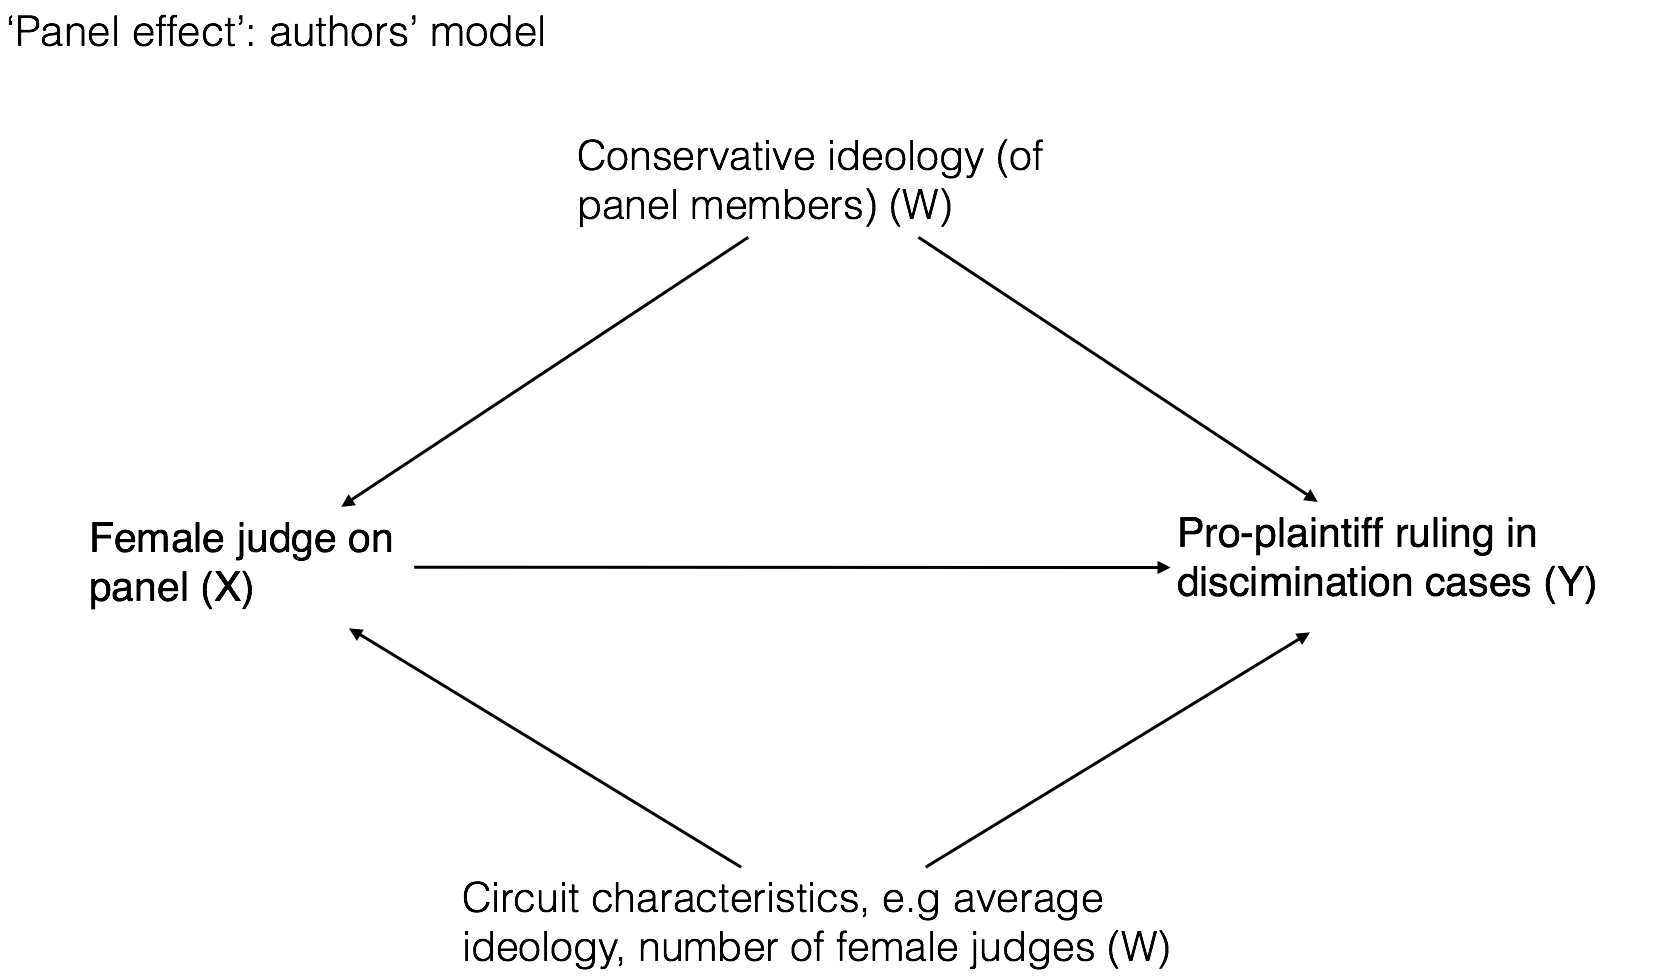
\includegraphics[height=.8\textheight,keepaspectratio=true]{../04-figures/06/08-w6_dag_full}
    \end{figure}
\end{frame}


\begin{frame}
	\frametitle{Boyd, Epstein, Martin \citeyear{boyd_untangling_2010}: Choosing controls}
	\footnotesize
  	 \begin{figure} 
    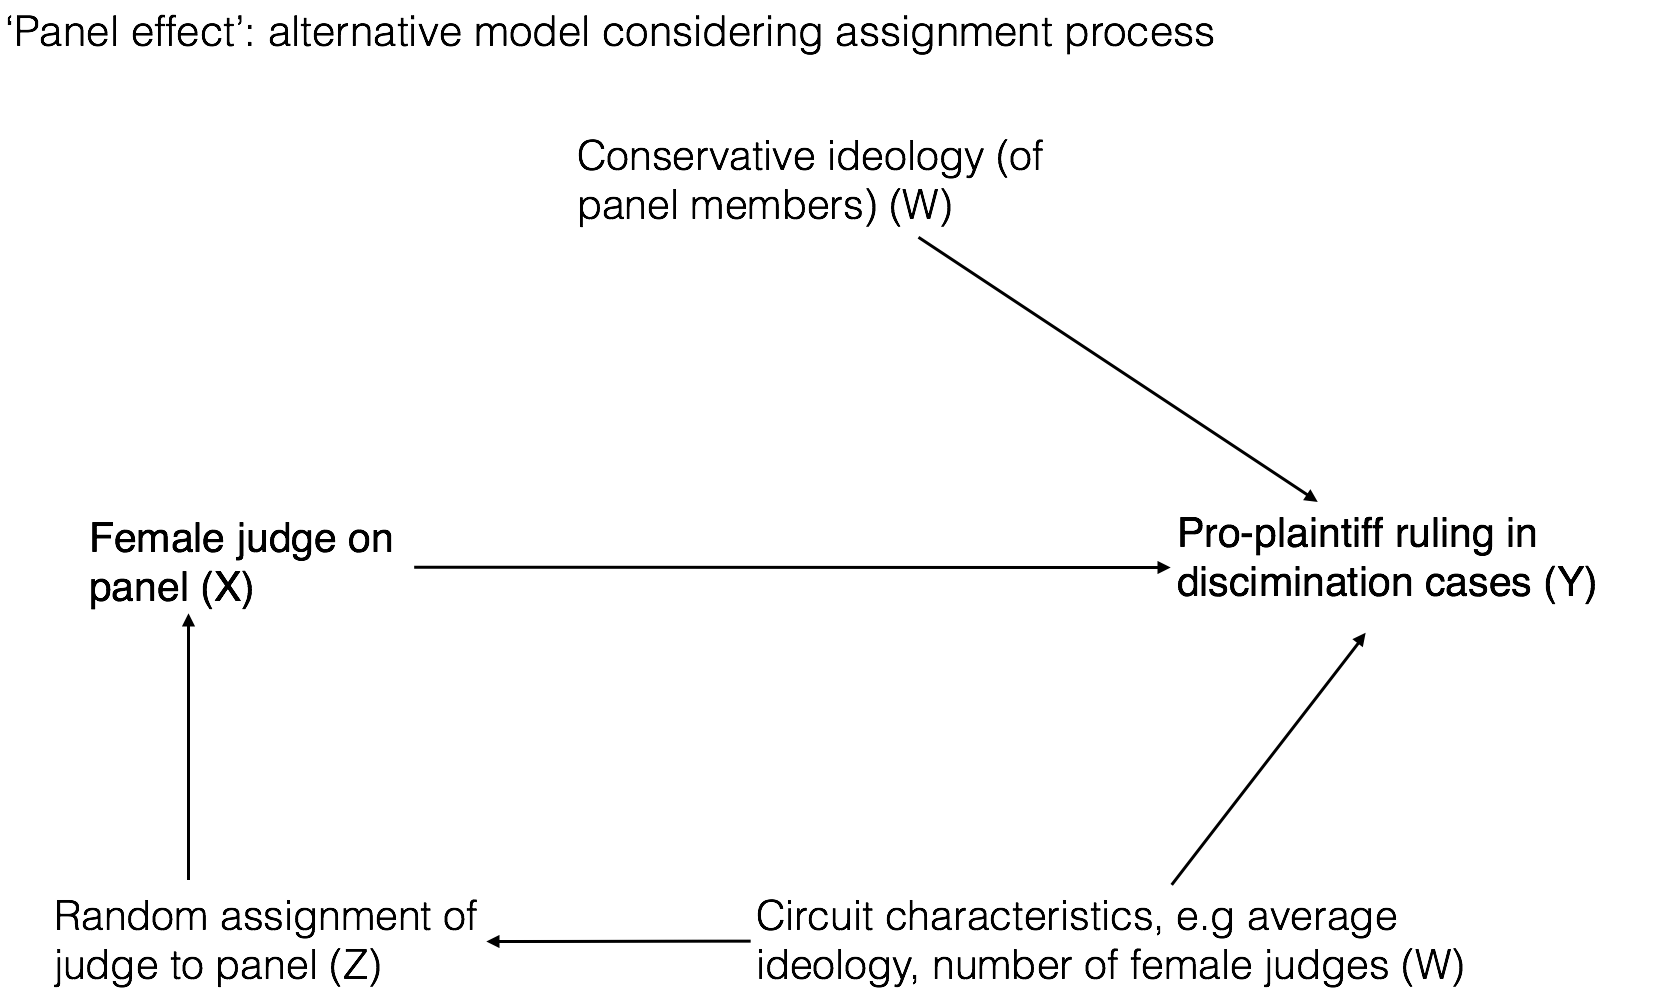
\includegraphics[height=.8\textheight,keepaspectratio=true]{../04-figures/06/09-w6_dag_random}
    \end{figure}
\end{frame}



\begin{frame}
	\frametitle{Boyd, Epstein, Martin \citeyear{boyd_untangling_2010}: Choosing controls}
	\footnotesize
  Results: compare regression and matched results
  	 \begin{figure} 
    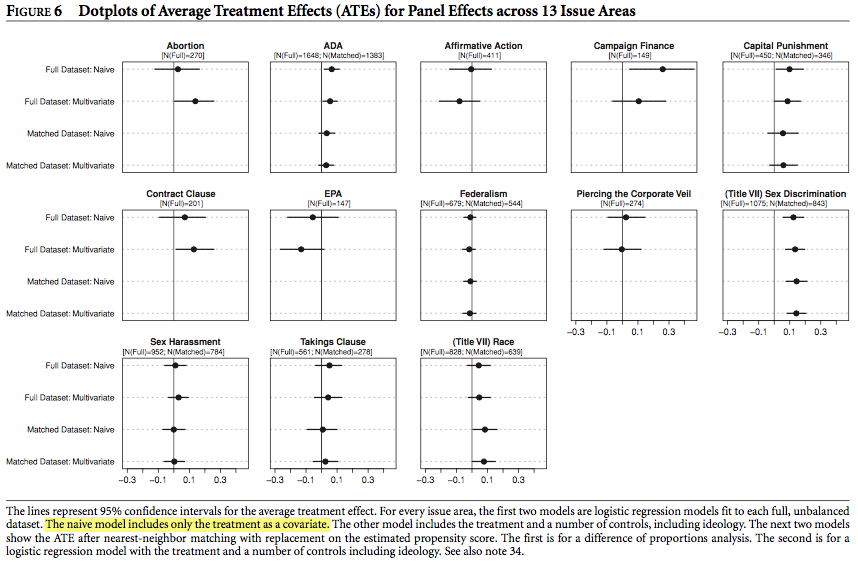
\includegraphics[height=.5\textheight,keepaspectratio=true]{../04-figures/06/10-w6_results}
    \end{figure}
    \tiny
    Results: 1. Naive model, 2. full controls, 3. PS, 4. PS with controls
    
    \scriptsize
    Given judges are assigned at random to panels, no big differences to be expected; most important effect probably from matching on circuit fixed effects, which the regression models do not control for
\end{frame}


\begin{frame}
	\frametitle{Boyd, Epstein, Martin \citeyear{boyd_untangling_2010}: Choosing controls}
	\footnotesize
    Matching as a valuable pre-analysis procedure
  	 \begin{figure} 
    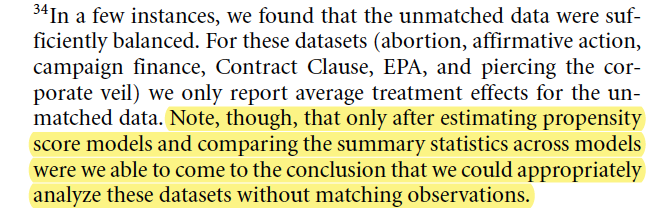
\includegraphics[height=.3\textheight,keepaspectratio=true]{../04-figures/06/11-w6_explanation}
    \end{figure}
\end{frame}


% END
\begin{frame}
\begin{center}
    \LARGE Thank you for watching, and see you next Monday!
\end{center}
\end{frame}

% REFERENCES %

\begin{frame}[allowframebreaks]
\frametitle{References}
\bibliographystyle{apacite}
\scriptsize\bibliography{../Bibliography}
\end{frame}

\end{document}
